%!TEX root = ../talk.tex

\section{Python}\label{sec:python}

%%%

\frameinlbffalse

{
\usebackgroundtemplate{
\tikz[overlay,remember picture] \node[opacity=0.8, xshift=-3cm, at=(current page.east)] {

\includegraphics[width=0.25\paperwidth]{figures/python_logo.jpg}
};}

\begin{frame}[plain]
\frametitle{\S\ref{sec:python}. \insertsection}
\listofframes
\end{frame}
\addtocounter{framenumber}{-1} % this page does not count

}

\frameinlbftrue


%%%
\subsection{A short introduction on Python}
%%%

\begin{frame}
  \MyLogo
  \frametitle{Python Language}  

\small 

\begin{itemize}

\item Created by Guido van Rossum in 1989 and first released in 1991

\item Named after ``the Monty Python'' (British comedy group)

\item An interpreted language---simple, clear, and readable 

\item Python has many excellent packages for machine learning

\item The language of choice in introductory programming courses

\end{itemize}

\begin{figure}[htbp] %  figure placement: here, top, bottom, or page
   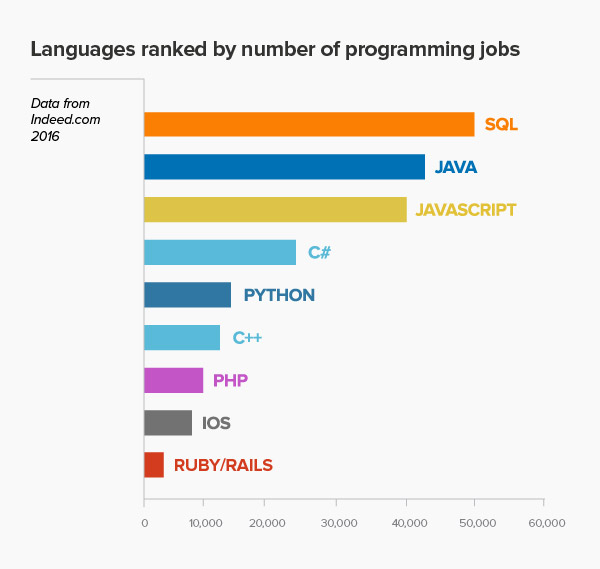
\includegraphics[height=1.7in]{figures/ComputerLanguagesDemand.jpg} 
   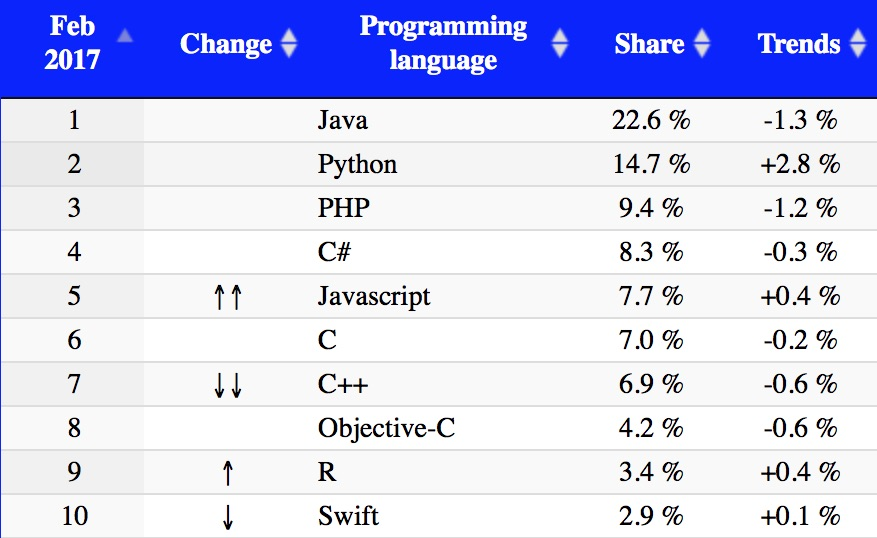
\includegraphics[height=1.7in]{figures/ComputerLanguagesShare.jpg} 
\end{figure}

\end{frame}

%%%

\begin{frame}
  \MyLogo
  \frametitle{Python for Scientific Computing}  

\small
\smallskip
\structure{Why Python for scientific computing?}
\begin{itemize}
	\item Dynamic data types and automatic memory management
	\item Full modularity, supporting hierarchical packages
	\item Strong introspection capabilities\footnote[frame]{\scriptsize\color{PineGreen}Code introspection is the ability to examine objects to know what they are, what they do and what they know. Python provides several utilities for code introspection, e.g. dir(), help(), type().}
	\item Exception-based error handling
\end{itemize}

\structure{Why consider such a slow language for simulation?}
\begin{itemize}
	\item Code readability and maintenance --- \alert{short code, fewer bugs}
	\item Good for proof-of-concept prototyping
	\item Implementation time versus execution time
	\item Well-written Python code is ``fast enough'' for most computational tasks
	\item Time critical parts executed through compiled language or \alert{available packages}
\end{itemize}

\end{frame}

%%%
\subsection{Basic language components}
%%%

\begin{frame}[fragile]
  \MyLogo
  \frametitle{Built-in Data Structures}  
\small

\smallskip
\structure{Numeric types: int, float, complex}
\begin{lstlisting}[language=python]
a=1	    # int
b=1L 	# long int
c=0xf	# int (hex format)
d=010	# int (octal format)
e=1.0	# float
f=1+2j	# complex
\end{lstlisting}

\structure{Sequence types: list, tuple, str, dict}
\begin{lstlisting}[language=python]
t=(3.14, True, 'Yes', [1], (0xf,))                # tuple example
l=[3.14, True, 'Yes', [1], (1L, 0xf)] + [None]*3  # list example
s='Hello' + ", " + 'world!'                       # str example 1
s=("Hello, " "world!")                            # str example 2
d={1: 'int', 'pi': 3.14}                          # dict example
s="Python"; s.find('thon')                        # find substring
\end{lstlisting}

\structure{Formatted output}
\begin{lstlisting}[language=python]
print('%(lang)s has %(num)02d quote types.' %{"lang":"Python", "num":3})
\end{lstlisting}

\structure{User defined functions}\footnote[frame]{\scriptsize\color{PineGreen}Function overhead is high. Not to call a function repeatedly; Using aggregation instead.}\footnote[frame]{\scriptsize\color{PineGreen}Python always passes (the value of) the reference to the object to the function.}

\begin{lstlisting}[language=python]
def square(x):
	return x*x
\end{lstlisting}

\end{frame}

%%%

\begin{frame}[fragile]
  \MyLogo
  \frametitle{Control Flow}  
\small

\medskip
\structure{If-then-else}
\begin{lstlisting}[language=python]
a = 1
if a > 0:
	print "a is positive"
elif a=0:
	print "a is zero"
else:
	print "a is negative"
\end{lstlisting}			

\structure{For loop}
\begin{lstlisting}[language=python]
# loop from 0 to 9
for i in range(10):
	print i
	
# loop over the list named by oldlist
newlist = [s.upper() for s in oldlist]

a = range(5)              # create a new list a = [0,1,2,3,4]
b = a                     # b points to the list a
c = [item for item in a]  # copy list a to a new list
\end{lstlisting}	
	
\structure{While loop}
\begin{lstlisting}[language=python]
sum = 0; i = 0
while i < 10:
	sum += i
	i += 1
\end{lstlisting}

\end{frame}

%%%

\begin{frame}[fragile]
  \MyLogo
  \frametitle{Modules}  
\small		

\begin{itemize}
\item This way will only introduce the module name into the name space in which the import command was issued. The names within the module will not appear in the enclosing namespace: they must be accessed through the module name.
\begin{lstlisting}[language=python,numbers=none] 
import math
math.sin(3.14)
\end{lstlisting}

\item This way does not introduce the name math into the current namespace. It does  introduce all public names of the math module into the current namespace.\begin{lstlisting}[language=python,numbers=none] 
from math import *
sin(3.14)
\end{lstlisting}

\item This will only import the sin function from math module and introduce the name sin into the current namespace, but it will not introduce the name math into the current namespace, directly use
\begin{lstlisting}[language=python,numbers=none] 
from math import sin
sin(3.14)
\end{lstlisting}

\item Make it as local as possible to avoid import overhead; But avoid calling it repeatedly; \alert{If possible, avoid it!}
\end{itemize}

\end{frame}

%%%

\begin{frame}[fragile]
	\MyLogo
	\frametitle{Additional Comments}  
	\small
	
\begin{enumerate}

\item In Python, everything (including functions, modules, and files) are objects. A variable is created through assignment:
\begin{lstlisting}[language=python,numbers=none] 
x = y = z = 0.1
\end{lstlisting}
				
\item help() is a function which gives information about the object. For example, 
\begin{lstlisting}[language=python,numbers=none] 
help('modules')       # generate a list of all modules that can be imported
help('modules time')  # generate a list of modules with 'time' in description
\end{lstlisting}
		
\item Use a profiler to find optimization possibilities
\begin{lstlisting}[language=python,numbers=none] 
import profile        # cProfile is now recommended
profile.run('main()')
\end{lstlisting}

\item Some useful and important packages
	\begin{itemize}\setlength\itemsep{0.25em}
	\item NumPy: for scientific computing
	\item Matplotlib: for visualising data
	\item SciPy: providing lots of numerical algorithms
	\item SymPy: for symbolic mathematics
	\end{itemize}
		
\end{enumerate}

\centering{\color{red}\scriptsize
\url{http://www.pythontutor.com}}

\end{frame}

%%%

\begin{frame}[fragile]
	\MyLogo
	\frametitle{Visualization}  
	\small

\vskip -12pt
\begin{columns}
\column{.5\textwidth}
\tiny{
\begin{lstlisting}[language=python]
# import pyplot module for visualization
import matplotlib.pyplot as plt
import numpy as np

# generate points (x,y)
dx = 0.001
x = np.arange(0, 2*np.pi, dx)
y = 0.1*np.sin(2*np.pi*x)

# plot (x,y) curve
plt.plot(x, y)
plt.show()	
\end{lstlisting}
}
\column{.45\textwidth}
%
\begin{figure}[htbp] 
   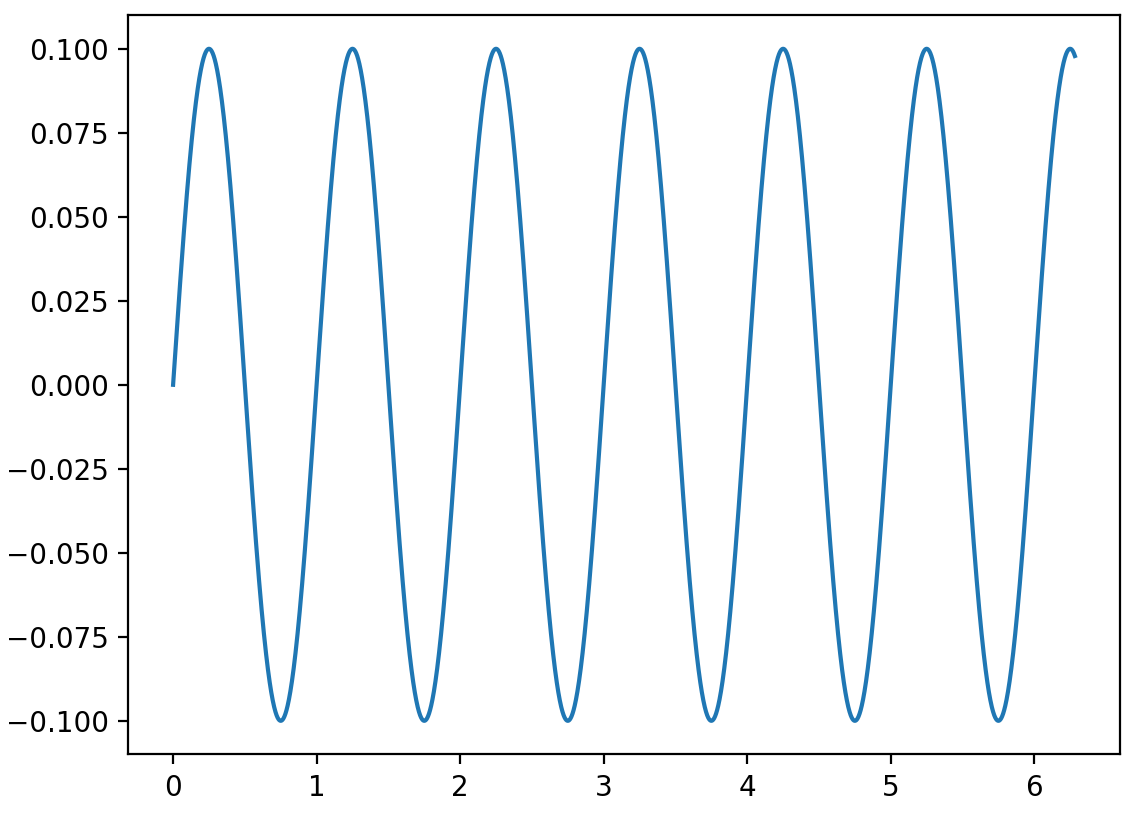
\includegraphics[width=0.95\textwidth]{figures/sin.png} 
\end{figure}
%
\end{columns}

\vskip -15pt
\begin{columns}
\column{.5\textwidth}
\tiny{
\begin{lstlisting}[language=python]
from mpl_toolkits.mplot3d import Axes3D
import matplotlib.pyplot as plt
from matplotlib import cm
import numpy as np

X = np.arange(-5, 5, 0.01)
Y = np.arange(-5, 5, 0.01)
X, Y = np.meshgrid(X, Y)
R = np.sqrt(X**2 + Y**2)
Z = np.sin(R)

# Plot the surface
fig = plt.figure()
ax = fig.gca(projection='3d')
surf = ax.plot_surface(X, Y, Z, 
                       cmap=cm.coolwarm)
plt.show()\end{lstlisting}
}
\column{.45\textwidth}
%
\begin{figure}[htbp] 
   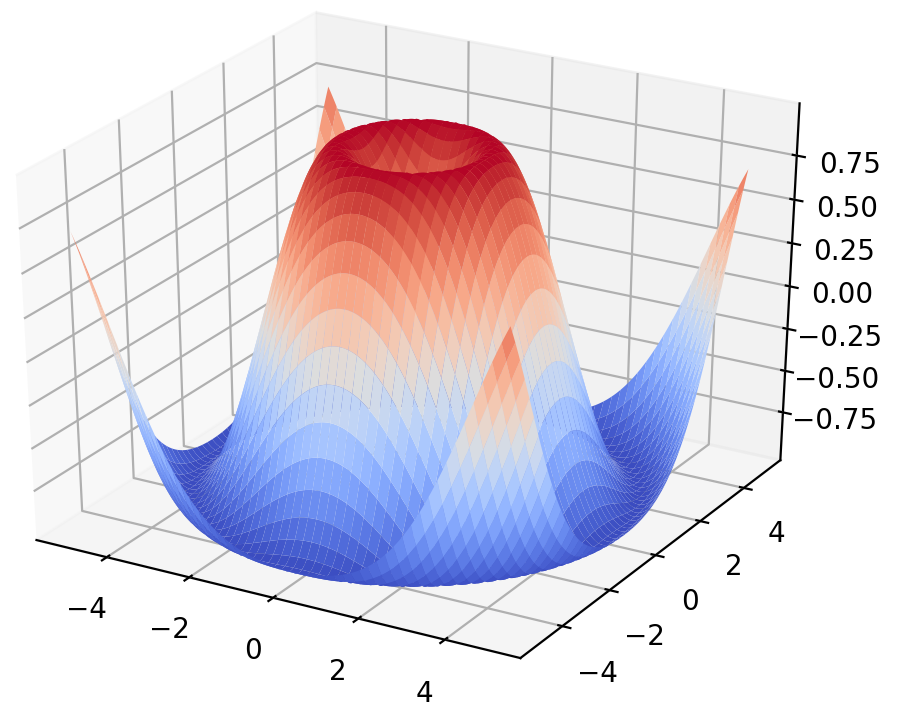
\includegraphics[width=0.95\textwidth]{figures/sin3D.png} 
\end{figure}
%
\end{columns}

\end{frame}